\documentclass{beamer}

\usepackage{graphicx}

\title{Integrating a secondary constraint into SAIL to generate wheelcases that allow for more freedom} 
\author[Jan Kruska]{Jan Kruska}
\date{12.02.2020}

%
%    \setbeamertemplate{footline}{%
%	\raisebox{5pt}{\makebox[\paperwidth]{\hfill\makebox[10pt]{\scriptsize\insertframenumber/\inserttotalframenumber}}}}

\setbeamertemplate{frametitle}{\nointerlineskip  
	\begin{beamercolorbox}[wd=\paperwidth,ht=2.75ex,dp=1.375ex]{frametitle}
		\hspace*{2ex}\insertframetitle \hfill {\scriptsize\insertframenumber/\inserttotalframenumber} \hspace*{1ex}%
	\end{beamercolorbox}}

\begin{document}

\begin{frame}{}
	\titlepage
\end{frame}

\frame{\tableofcontents}

\section{Problem}
\frame{\frametitle{Problem}
	\begin{block}{Problem}
		The existing wheelcase inhibits the maximum steering angle of the wheels
	\end{block}
	\begin{itemize}
		\item Generate wheelcases that do not inhibit wheel movement while still maintaining some aerodynamic optimality
	\end{itemize}
}
\section{Method}
\frame{\frametitle{SAIL}
%SAIL is a surrogate assisted phenotypically divergent version of the genetic algorithm MAP-Elites.
%\begin{itemize}
%	\item Phenotypically divergent, it produces a diverse set of individuals, more specifically a map that is divided along phenotypic categories.
%	\item Surrogate assisted, it makes use of a gaussian process as a surrogate to reduce the number of needed Evaluations of the real fitness function.
%\end{itemize}
\begin{figure}
	\centering
	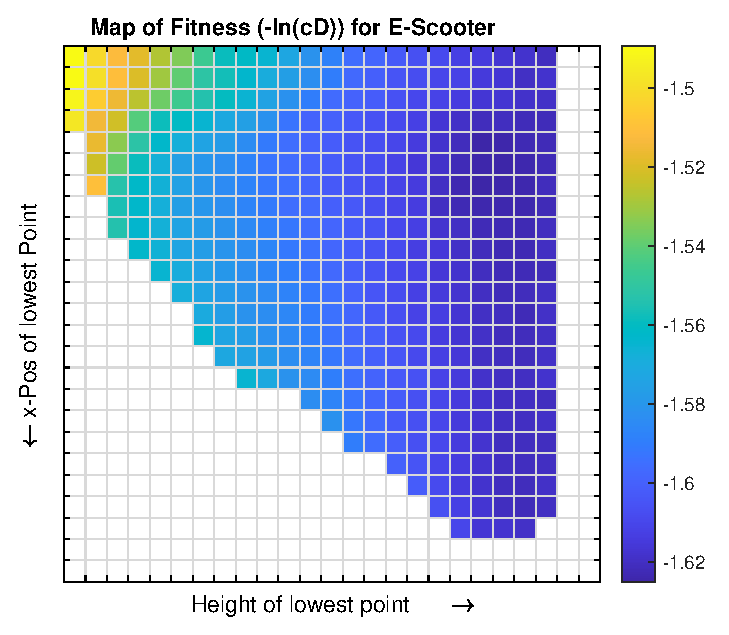
\includegraphics[width=.7\linewidth]{../thesis/bilder/escooter/dragMapEscooter}
\end{figure}

}
\frame{\frametitle{Categorization}
	\begin{itemize}
		\item MAP-Elites needs Categories to assign individuals their respective cells
		\item Currently the chosen Categories are:
		\begin{enumerate}
			\item Width of the velomobil
			\item x-Position of the widest Point\footnote{The velomobil is directed towards -X, so bigger values correspond to the widest point being further back}
		\end{enumerate}
	\end{itemize}
}
\frame{\frametitle{Free Form Deformation}
	\begin{figure}[h]
		\centering
		\begin{minipage}{0.45\textwidth}
			\centering
			\includegraphics[width=1\linewidth]{../thesis/bilder/sphere_lattice}
%			\caption{3D-Mesh einer Kugel in 4x4x4 FFD-Box}
			\label{fig:ffd_undeformed}
		\end{minipage}\hfill
		\begin{minipage}{0.45\textwidth}
			\centering
			\includegraphics[width=1\linewidth]{../thesis/bilder/sphere_lattice_deformed2}
%			\caption{Deformiertes 3D-Mesh ezeugt durch Bewegung der Deformationspunkte}
			\label{fig:ffd_deformed}
		\end{minipage}
	\end{figure}
}
\frame{\frametitle{Soft Constraint vs. Hard Constraint}
	\begin{itemize}
		\item Two different solutions, which both violate the constraint, can still differ in terms of the severity of the violation
		\item The current wheelcase does violate the constraint, so at the beginning of the process no non-trivial solution, that fulfills the constraint, is known
		\item Because of those two considerations a soft constraint, seemed more useful for the problem at hand
	\end{itemize}
}

%\frame{\frametitle{Modeling of the Constraint}
%\begin{itemize}
%	\item Due to the number of times the constraint has to be evaluated, the calculation needs to be reasonably fast
%\end{itemize}
%}

\frame{\frametitle{Steering Volume}
	The space needed by the wheel for all possible steering angles can be modeled as a volume:
	\begin{figure}
		\includegraphics[width=1\linewidth]{../thesis/bilder/radausschlag.png}
	\end{figure}
}

\frame{\frametitle{Constraint + Velomobil}
	This volume intersect with the current wheelcase 
	\begin{figure}
		\includegraphics[width=1\linewidth]{../thesis/bilder/radausschlag_inclVelo.png}
	\end{figure}
}

\frame{\frametitle{Constraint Volume}
	The Constraint can be calculated as the volume outside of the wheelcase, using mesh-difference operation
	\begin{figure}
		\includegraphics[width=1\linewidth]{../thesis/bilder/difference.png}
	\end{figure}
	This does not perfectly map to the real constraint, but it is stipulated, that the volume outside of the wheelcase is negatively correlated with the largest possible steering angle.
}

\section{Results}
\frame{\frametitle{SAIL-Parameters}
	\begin{enumerate}
		\item Real Evaluations: 1000
		\item Generations Acquisition: 2048
		\item Generations result: 8192
		\item Children per Gen : 32
		\item Map-resolution: 25x25
	\end{enumerate}
%	\begin{table}[h]
%		\centering
%		\begin{tabular}{.75\textwidth}{ll}\hline
%			Anzahl initialer Samples & 100 \\
%			%\rowcolor{lightgray}
%			Anzahl Samples & 1000 \\
%			Anzahl neuer Samples pro Akquiseschleife & 20 \\
%			%\rowcolor{lightgray}
%			Anzahl Generationen Akquise-MAP-Elites & 2048 \\
%			Kinder pro Generation Akquise-MAP-Elites & 32 \\
%			%\rowcolor{lightgray}
%			Anzahl Generationen Ergebnis-MAP-Elites & 8192 \\
%			Kinder pro Generation Akquise-MAP-Elites & 32 \\
%			Auflösung der MAP-Elites Karte & 25 * 25  \\
%			\hline
%			Freiheitsgrade & 18 \\
%			Mittelwertgewichtung & 1 \\
%			Varianzgewichtung & 2 \\
%			Constraintgewichtung & 1 \\
%		\end{tabular}
%		\label{tab:params3rd}
%		\caption{Parametrisierung des dritten Experiments (Änderungen zum zweiten Experiment hervorgehoben)}
%	\end{table}
}
\frame{\frametitle{FFD-Configuration}
	\begin{figure}
		\centering
		\includegraphics[width=.7\linewidth]{../thesis/bilder/6ptDeformationPoints.png}
	\end{figure}
}
\frame{\frametitle{Comparison non-constrained vs. constrained}
	\vspace*{\fill}
\begin{figure}[h]
	\centering
	\begin{minipage}{0.45\textwidth}
		\centering
		\includegraphics[width=1\linewidth]{../thesis/bilder/6pt1000Samples/dragBoxplot}
%		\caption{Comparison of final drag values}
		\label{fig:3rddragbox}
	\end{minipage}\hfill
	\begin{minipage}{0.45\textwidth}
		\centering
		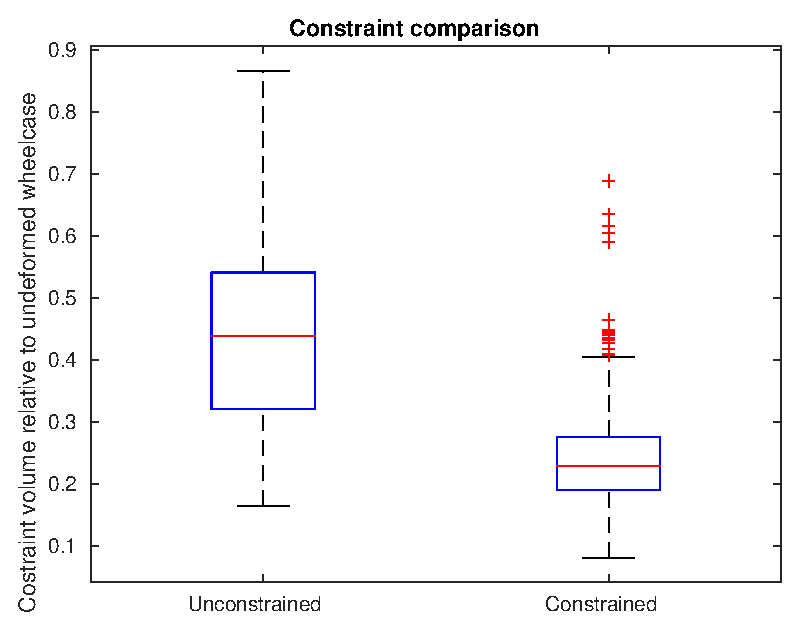
\includegraphics[width=1\linewidth]{../thesis/bilder/6pt1000Samples/constraintBoxplot}
%		\caption{Comparison of final constraint values}
		\label{fig:3rdconbox}
	\end{minipage}
\end{figure}
}

\frame{\frametitle{Drag-maps}
\begin{figure}[h]
	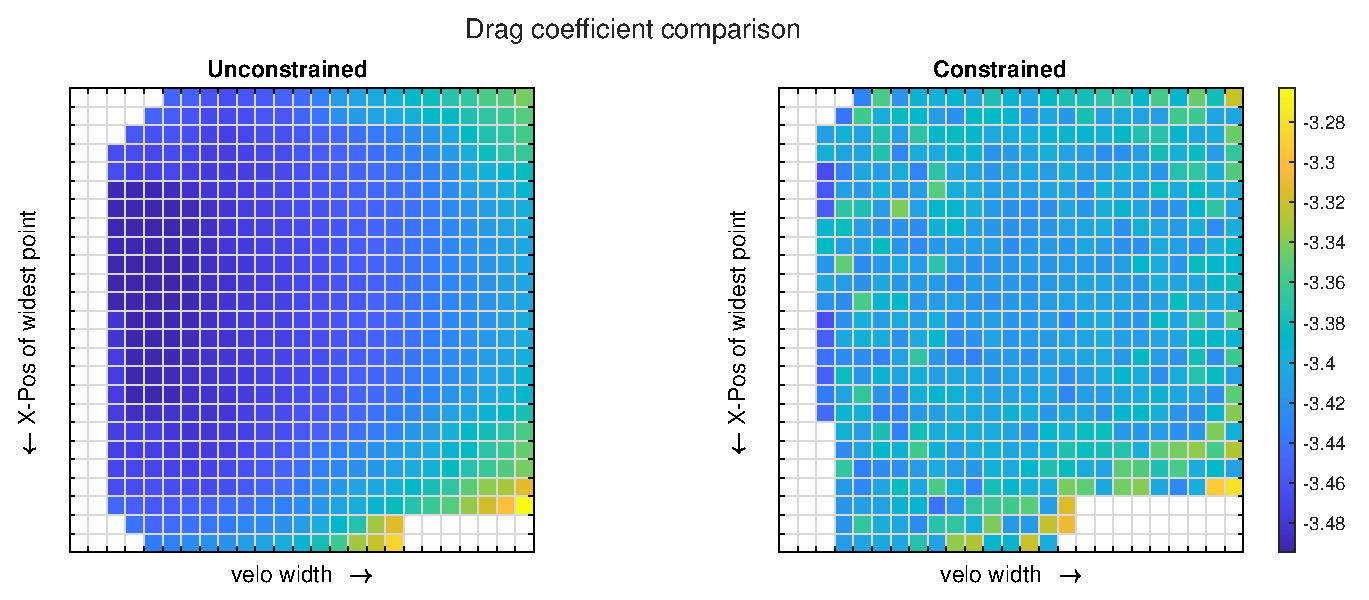
\includegraphics[width=1\linewidth]{../thesis/bilder/6pt1000Samples/dragMapComparison}
	\caption{Maps of final drag values}
	\label{fig:3rdmapDrag}
\end{figure}
}

\frame{\frametitle{Constraint-maps}
	\begin{figure}[h]
		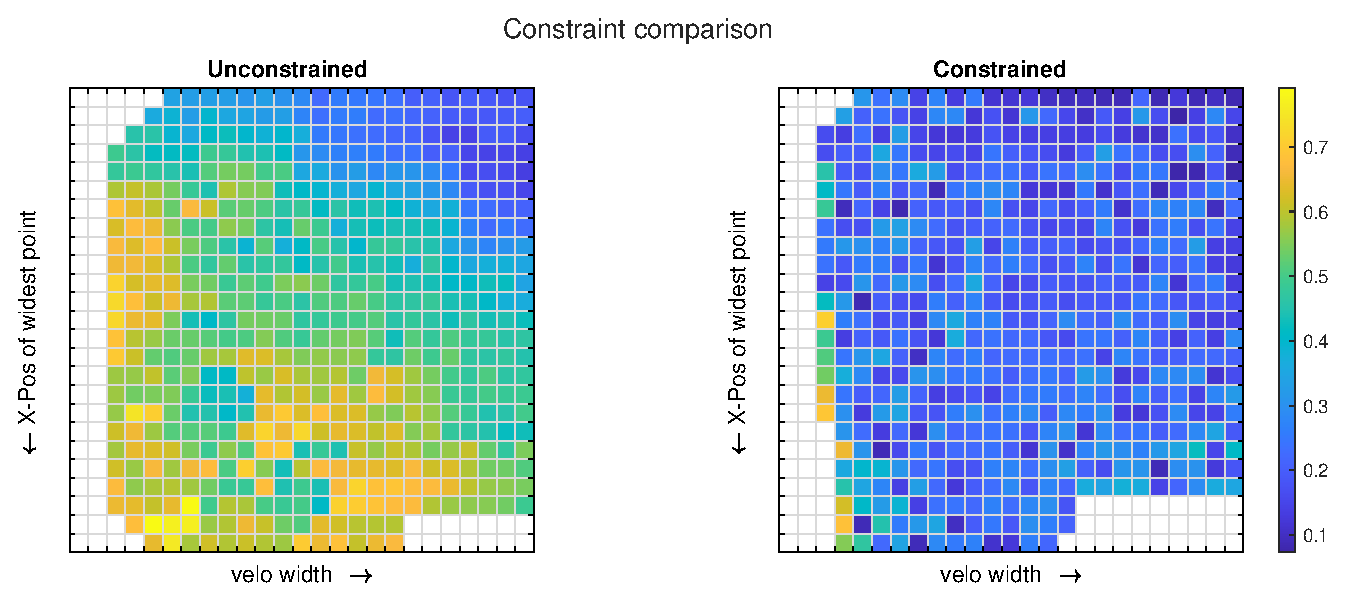
\includegraphics[width=1\linewidth]{../thesis/bilder/6pt1000Samples/constraintMapComparison}
		\caption{Maps of final constraint values}
		\label{fig:3rdmapCon}
	\end{figure}
}

\frame{\frametitle{Top down comparison}
\begin{figure}[h]
	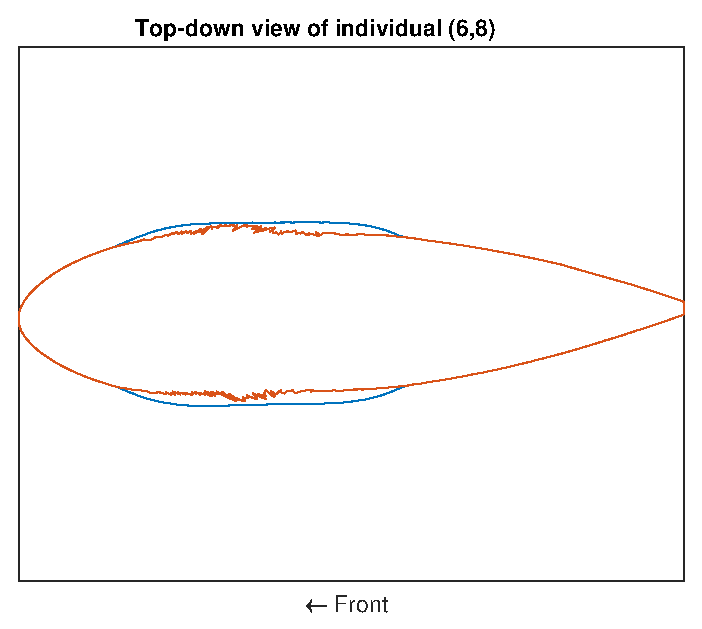
\includegraphics[width=1\linewidth]{topdown}
\end{figure}
}

\frame{\frametitle{Unconstrained}
	\begin{figure}[h]
		\includegraphics[width=1\linewidth]{6_8_uncon}
	\end{figure}
%	cD = 0.0304, width=580.22 mm,
}

\frame{\frametitle{Constrained}
	\begin{figure}[h]
		\includegraphics[width=1\linewidth]{6_8_con}
	\end{figure}
%cD = 0.0327, width=598.7912 mm, 
}

\frame{\frametitle{Discussion}
	\begin{itemize}
		\item The resulting cD Values are worse when using a constraint, yet that is to be expected.
		\item The algorithm works toward fulfilling the constraint, especially in areas in which that is harder
		\item However solutions that completely fulfill the constraint are still located in aerodynamically bad areas
		\item Improvements could be made in choosing a different FFD-Configuration, x-Deformations seem largely unimportant whereas y-Deformations of the top row seem very important
	\end{itemize}
}
%\section{Future experiments}
%\frame{\frametitle{Future changes}
%\begin{itemize}
%	\item Change FFD-parameters, to facilitate more degrees of freedom
%	\item Longer rund, more generations \& more OpenFoam Evaluations
%\end{itemize}
%}


\end{document}
